\section{Sanity check}
%%% TODO: Build bridge from previous chapter 
Having introduced our cell dynamics, we now want to take a look at the simulation results.
Therefore, we aim to compare our simulation results to results from an established cell model from \cite{Bruna2012}. 
In \cite{Bruna2012} the diffusion dynamics of first a point particle model and second a hard sphere model is studied. 
Thereby, the two density distributions:
\begin{itemize}
    \item the joint probability density function $P(\vec{X}, t)$ of the system of all cell centres $\vec{X}$ at time $t$,
    \item the marginal distribution function of the first particle $p(\vec{x}_1, t)$
\end{itemize}
play an important roll. \\
The joint probability density function $P(\vec{X}, t)$ is a function describing the positions of all particles in the system, while the marginal distribution function $p(\vec{x}_1, t)$ is a function describing only the position of the first particle. \\
It is sufficient to consider only the marginal distribution function of first particle, because all particle act similarly. \\ 
Gaining $p(\vec{x}_1, t)$ from $P(\vec{X}, t)$ is a big reduction of complexity, since we reduce from a high-dimensional PDE for $P$ to a low-dimensional PDE for $p$. 
The marginal distribution function the of first particle can be computed via
\begin{center}
    $
    p(\vec{x}_1, t) = \int P(\vec{X}, t) d\vec{x}_2 \dots  d\vec{x}_N.
    $
\end{center} 

%%% TODO: introduce: Heat equation for point particles and explain model for this 
The most simple model that gets considered for the diffusion dynamics of cell systems is the point particle model. 
Here the cells get modeled with sizeless points that perform a Brownian motion on the domain. \\
Since the cells do not have a real size, no interaction between the cells can occur, since they will never hit upon each other.  

The paper\cite{Bruna2012} analyses these dynamics on the domain 
\begin{center}
    $
    \Omega_{\cite{Bruna2012}} = [-0.5, 0.5]^2,
    $
\end{center}
on which $400$ particles are located. \\
The particles are initially distributed according to a normal distribution with mean 0 and standard deviation 0.09. 
This initial distribution has an integral of one over $\Omega_{\cite{Bruna2012}}$. \\
The movement of each point particle $\vec{x}_i$ in the simulation is given by the stochastic differential equation (SDE)
\begin{center}
    $d \vec{x}_i = \sqrt{2} d B_i dt$, \hspace{0.5em}
    $1 \leq i \leq 400$,\hspace{0.5em}
    on $ \Omega_{\cite{Bruna2012}}$, \\
\end{center}
The reflective boundary condition on $\partial \Omega_{\cite{Bruna2012}}$ is imposed:
\begin{equation}
    \nabla_{\vec{x}} p \cdot \vec{n} = 0.
\end{equation}
It is known, that particles in this setup move according to the heat equation, i.e.
\begin{equation}
    \frac{\partial p}{\partial t}(\vec{x}_1, t) = \Delta_{\vec{x}_1} p = \nabla_{\vec{x}_1} \cdot [ \nabla_{\vec{x}_1} p]
    \label{eq:heat}
\end{equation}
inside of the domain. \\

A next step that results in the hard sphere cell model (HSCM) is to give the cell particles a real size. \\
Let $0 < \epsilon \ll 1$ be the diameter of all cells that are now two dimensional discs with the same size. 
This changes the dynamics of the cells immense, since they now have chance to collide into each other which is a form of interaction. \\
The authors of \cite{Bruna2012} also did a simulation with the HSCM. 
The setting is as similar as possible to the point particle model, because a main goal of the paper was to compare the diffusion characteristics of both models. 
There are still $400$ cells located on the domain. \\
But the first changes are already needed to be made in the initial condition.  
We do not want a setting where two cells overlap each other. 
Thus, the $400$ cells get initialized in the following way:
\begin{enumerate}
    \item Generate a point $\vec{x} ~ N(0,0.09)^2$. 
    \item If for all already generated centres $\vec{x}_j: \norm[\vec{x} - \vec{x}_j] > \epsilon$ is true, use $\vec{x}$ as the next cell centre, otherwise discard the point and restart with step 1 until $400$ cell centres are found.   
\end{enumerate}
Since we do not want any overlap to occur during the whole simulation, the feasible domain is given by $\Omega_{\cite{Bruna2012}}^{\epsilon}$ which is the subset of $\Omega_{\cite{Bruna2012}}$ that excludes all areas where there exists a cell centre that has a distance of less than $\epsilon$ to it. \\
The cells perform the same Brownian motion as the point particles. 
The next question is, how cell collisions are modeled. 
Let us assume that two cells $i$ and $j$ are given such that $\norm[\vec{x}_i - \vec{x}_j] = \epsilon$ is true. 
Then, both cell centres are located at the boundary $\partial \Omega_{\cite{Bruna2012}}^{\epsilon}$. 
Here, the reflective boundary condition is still imposed and it causes both cells to bounce of from each other in the direction of the outward normal vector from the excluded area of the respectively other cell. \\ 
We can note that the interaction does not come from any kind of interaction term that describes the dynamics of the cells inside of the domain, like in our model's approach.
But instead, the whole feasible domain changes with the moving cells in the HSCM and thus the domain's boundary changes where the reflective boundary condition causes all cells to bounce of. \\ 

In \cite{Bruna2012} the authors managed to compute the marginal distribution function of the first particle of the HSCM. 
In two dimensions it is given by:
\begin{equation}
    \frac{\partial p}{\partial t}(\vec{x}_1, t) = \nabla_{\vec{x}_1} \cdot \{\nabla_{\vec{x}_1}[p + \frac{\pi}{2}(400 - 1)\epsilon^2 p^2]\}.
    \label{eq:hard-sphere-p}
\end{equation}
We can see, that a positive term was added to the dynamics of the point particle model \ref{eq:heat}. 
That means that the bounce effect of the real sized hard spheres increases the diffusitivity of the cell system. 

Another evidence of this behavior is shown in Figure 2 in \cite{Bruna2012}. 
This figure contains the following four plots:
\begin{enumerate}[label=(\alph*)]
    \item shows the solution of the linear diffusion equation \ref{eq:heat} for point particles.
    \item shows the histogram of a Monte Carlo simulation of the point particle model.
    \item shows the solution of the nonlinear diffusion equation \ref{eq:hard-sphere-p} for finite-sized particles.
    \item shows the histogram of a Monte Carlo simulation of the HSCM. 
\end{enumerate} 
In a Monte Carlo simulation, a stochastic process is simulated many times in order to analyse whether the results follow a specific stochastic distribution.
In our case that specific stochastic distribution is the density 

%%% TODO: introduce: all further simulation properties of bruna12: Domain, Number of cells, Number of Simulations, Initial distribution, Diffusitivity constant, epsilon and cell radius, forces in new simulation, spatial discretisation, time interval, time step size, Number of Cell wall points
* 400 particles/cells 
* initial distribution ~ N(0,0.09) + no overlaps for hard discs 
The domain of the system is 

a square with side length $1$ around the origin
% TODO: discretisation parameters 
and the time step size is $10^-5$. 

%%% TODO: describe: principle of monte carlo simulation
%%% TODO: introduce: what does Figure 2 show?
Figure $2$ in \cite{Bruna2012} shows the marginal distribution function $p(x_1, t)$ at time $t = 0.05$. 
The figure compares the solution of the nonlinear diffusion equation $(11)$ for finite-sized particles with the solution of the linear diffusion equation $(4)$ for point particles. \\
The figure consists of four plots:

The figure is a useful tool for understanding the behavior of the system and the effects of excluded-volume interactions on the collective diffusion rate.
The the heat equation and Equation $(4)$ and in Figure $2a$ and $2c$ show similar characteristics as the stochastic simulations in $2b$ and $2d$. 
We can observe that the excluded-volume effects enhance the overall collective diffusion rate.
% TODO: ... as equation ... already indicated 

%%% TODO: tell that we want to test what our model delivers 
%%% TODO: explain all parameters from new model 
%%% TODO: name Julia framework that got used for solving the pde 
%%% TODO: conclude that we hopefully have matching results 



\begin{figure}[]
	\centering
    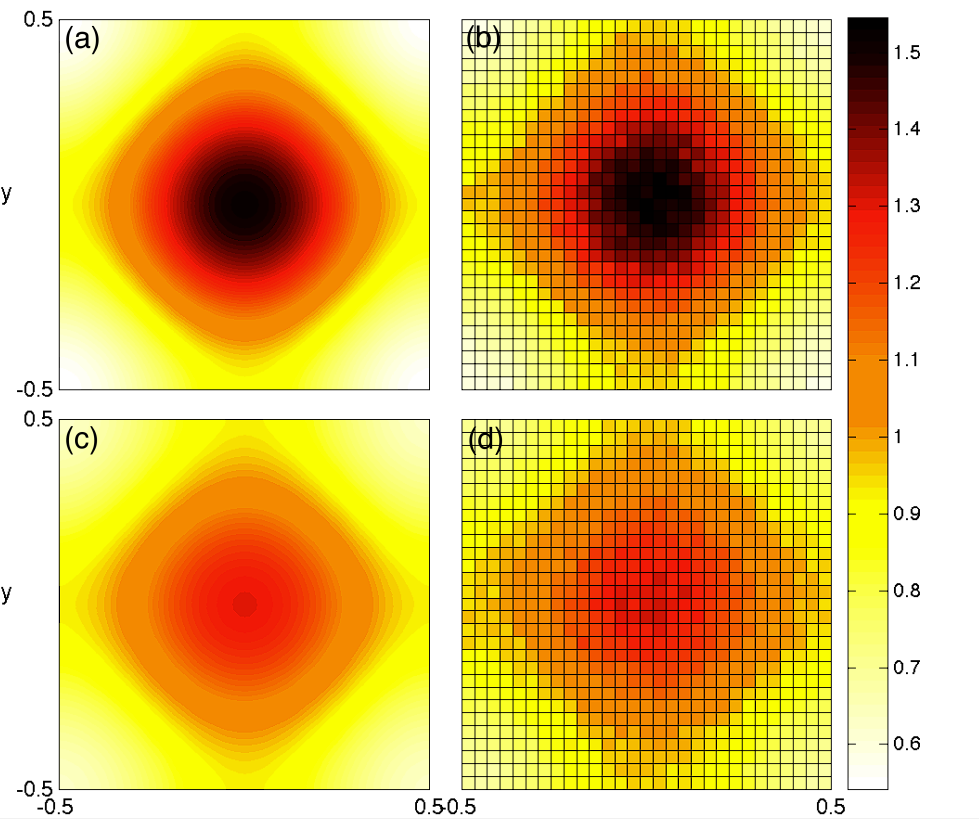
\includegraphics[width=\textwidth]{sanity-check/bruna12_theOriginal.png}
    % \caption{Plot from Bruna & Chapman 2012}
\end{figure}

% \begin{figure}[]
% 	\centering
% 	\begin{subfigure}{0.4\textwidth}
% 		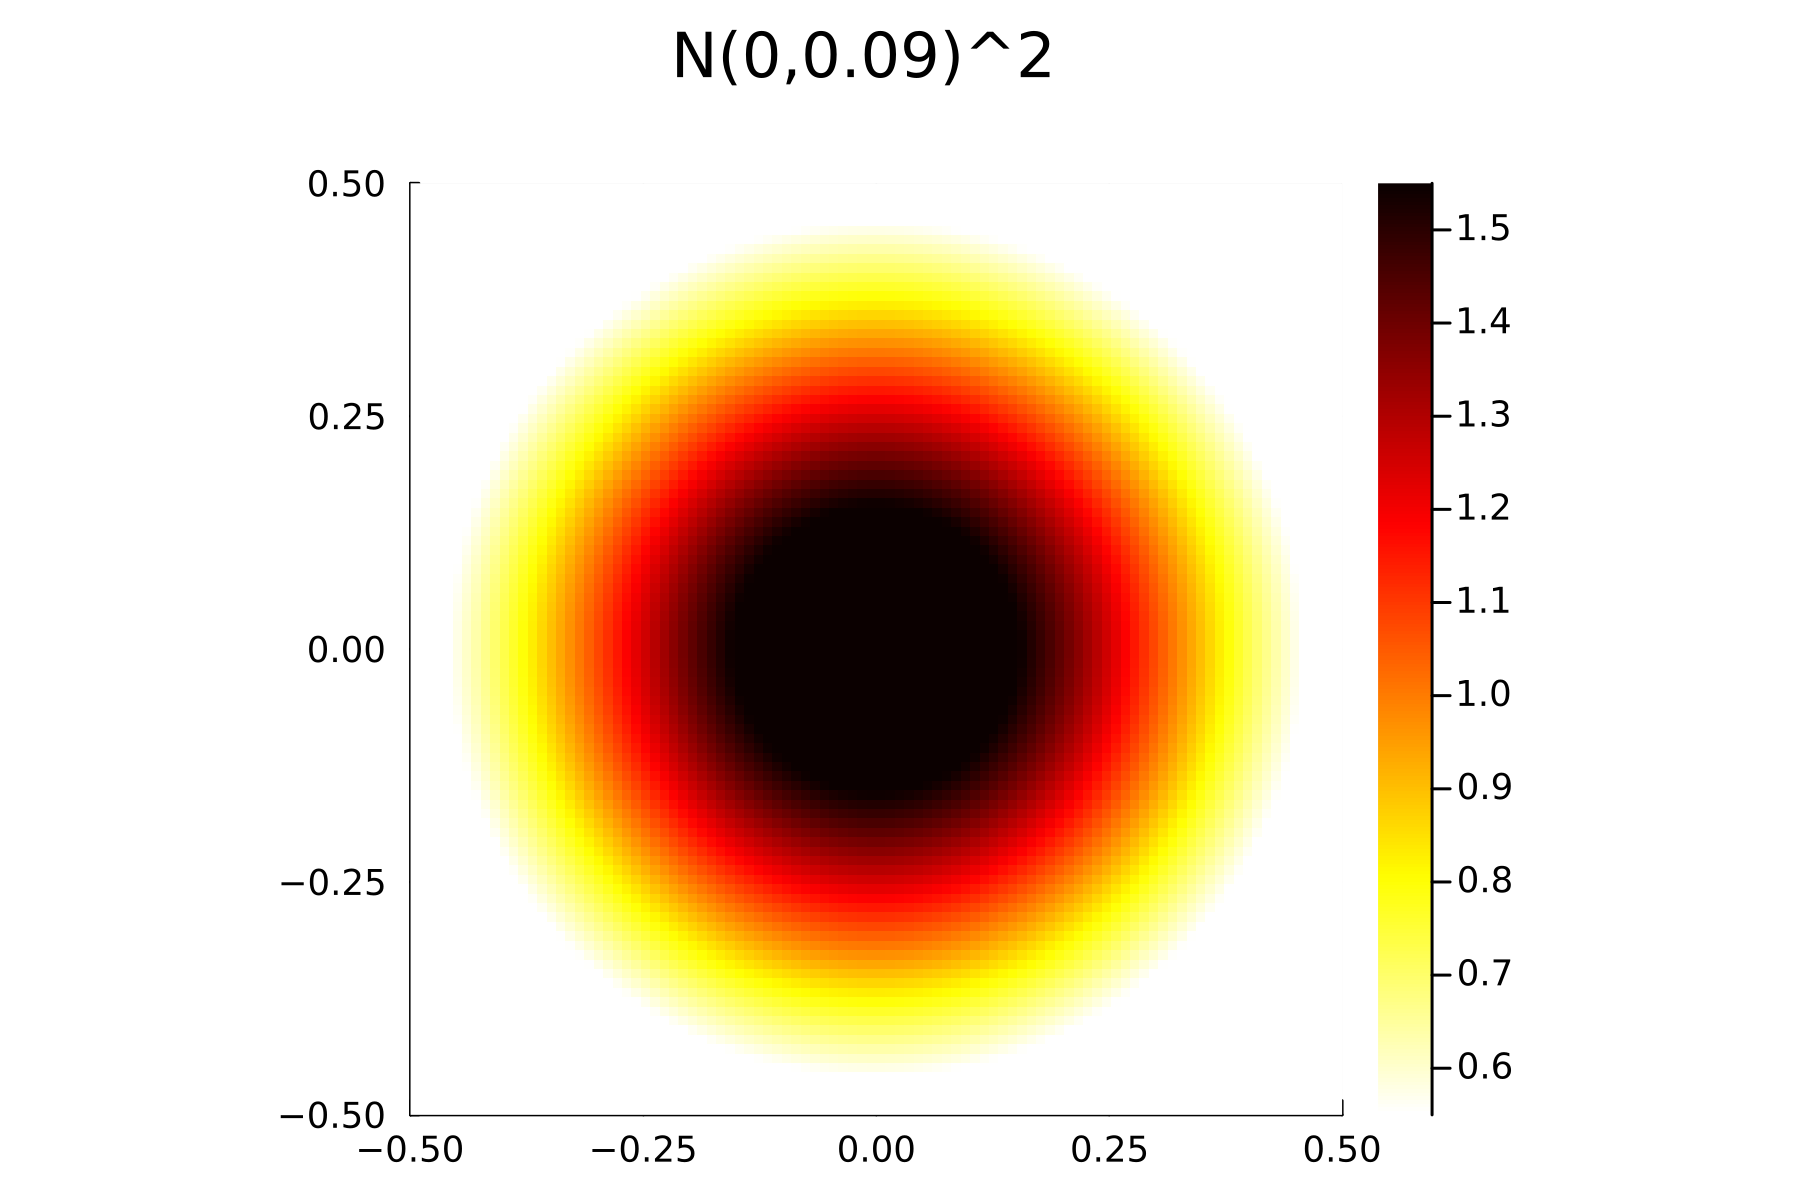
\includegraphics[width=\textwidth]{figures/sanity-check/bruna-scale/normal-distribution-bruna12-scale.png}
% 		\caption{}
% 	\end{subfigure}
%     \begin{subfigure}{0.4\textwidth}
% 		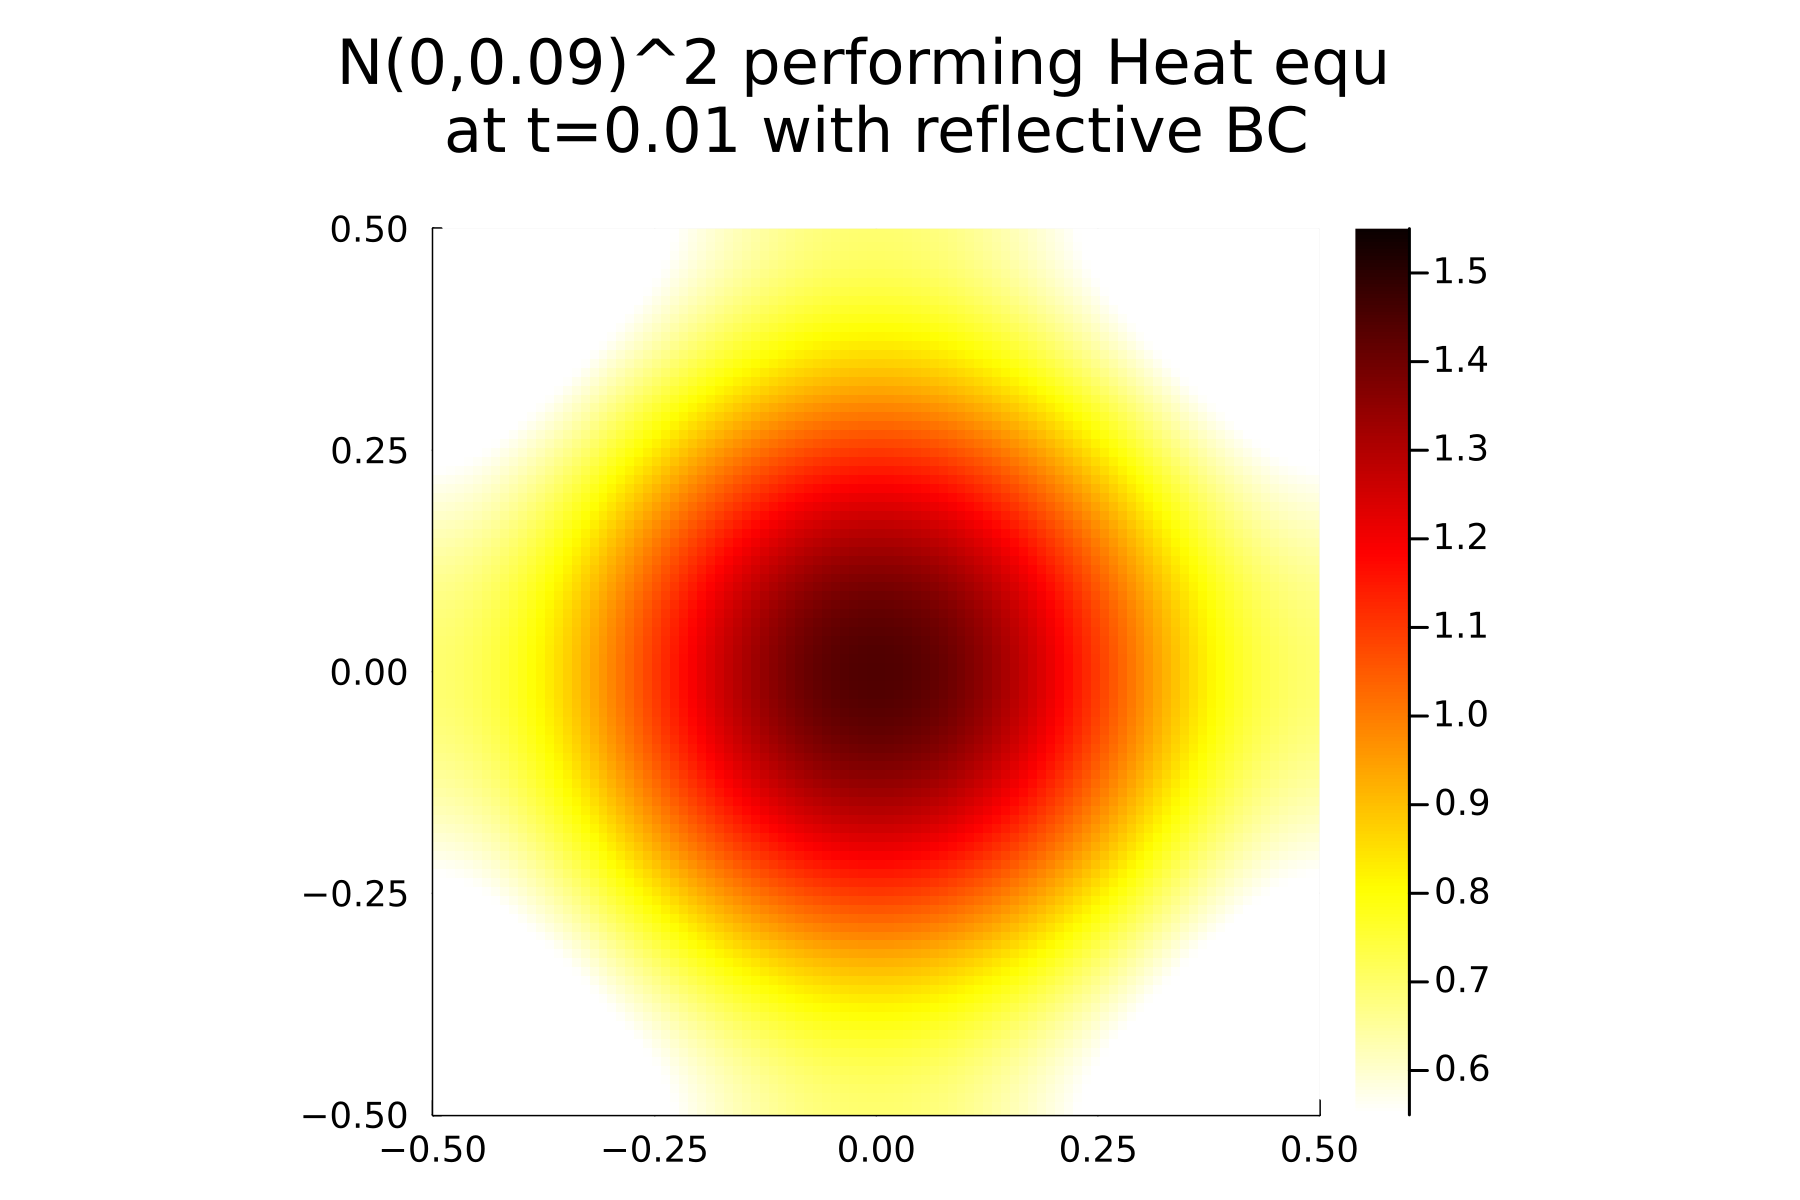
\includegraphics[width=\textwidth]{sanity-check/bruna-scale/heat-dynamic-bruna12-scale-T0-01.png}
% 		\caption{}
% 	\end{subfigure}
% 	\hfill
% 	\begin{subfigure}{0.4\textwidth}
% 		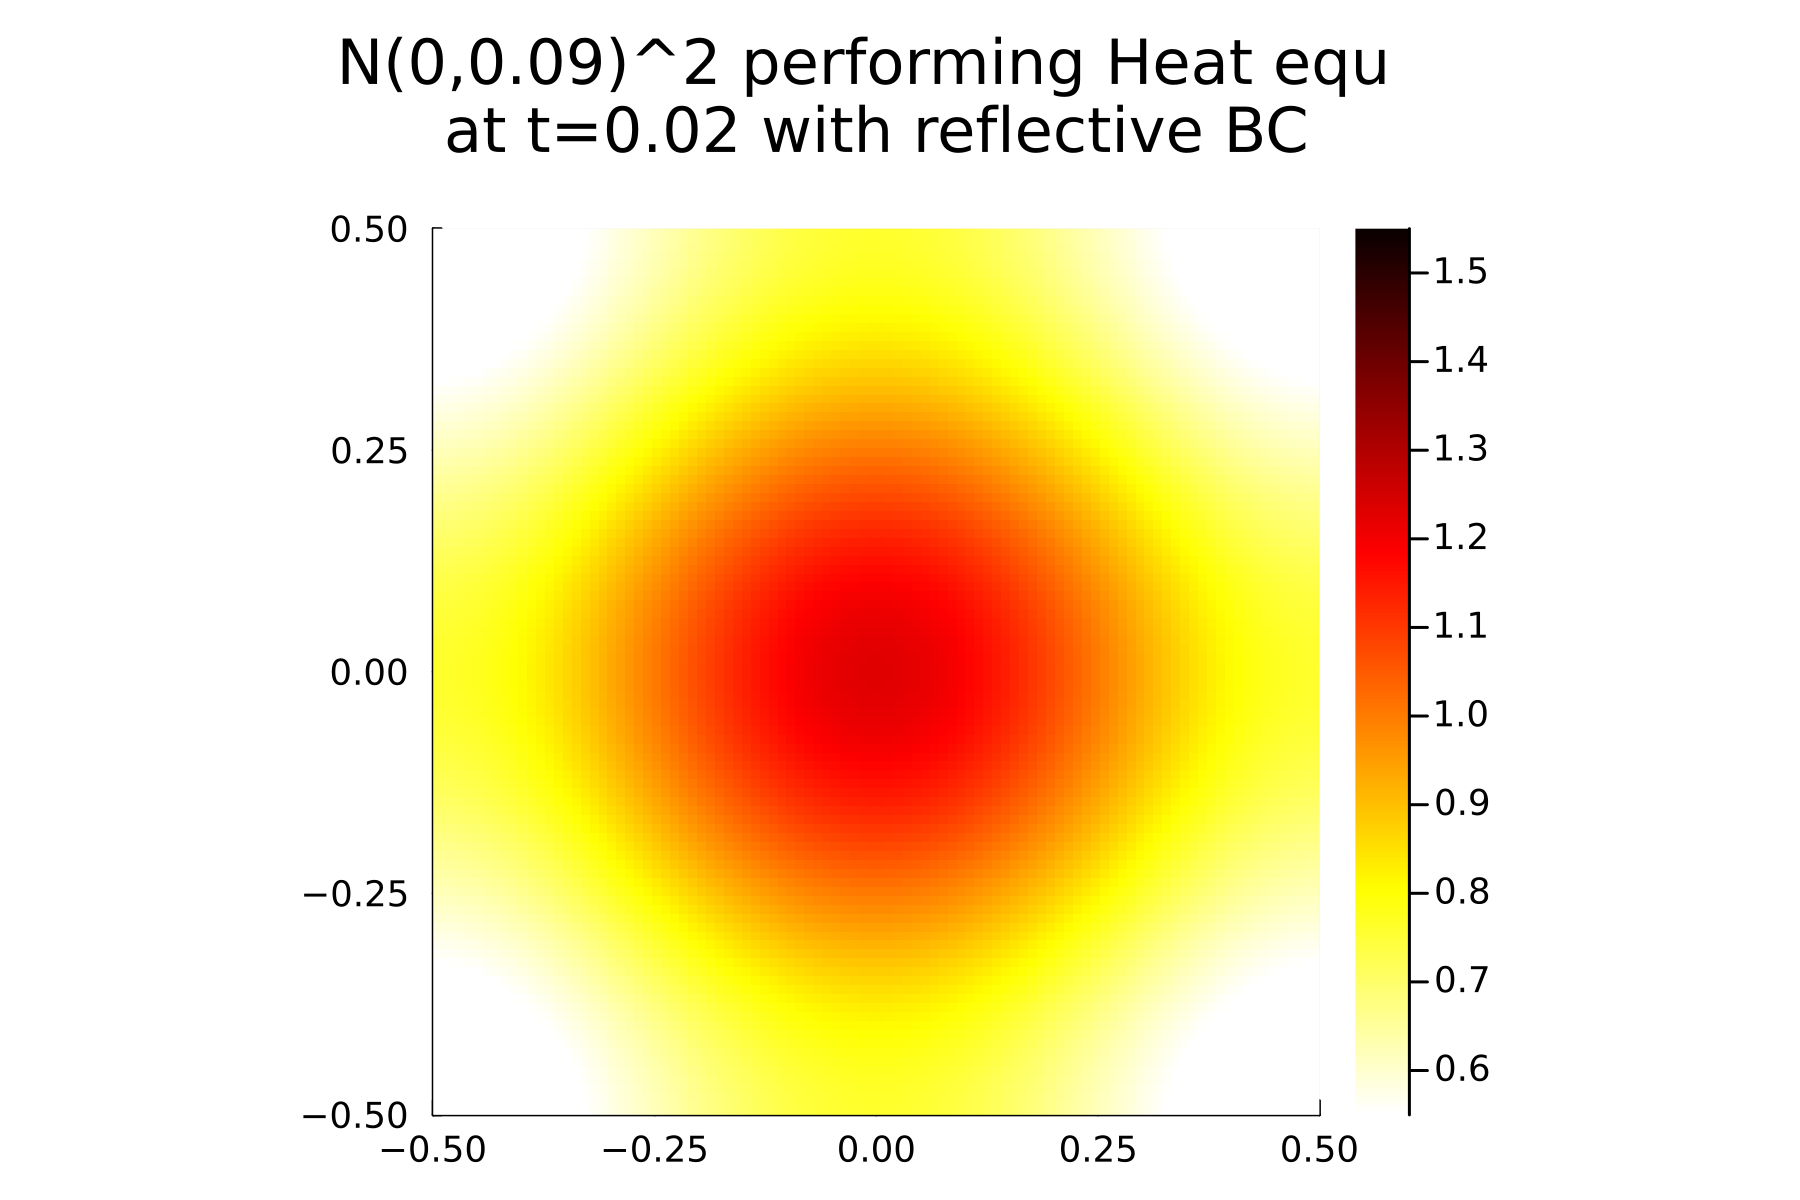
\includegraphics[width=\textwidth]{sanity-check/bruna-scale/heat-dynamic-bruna12-scale-T0-02.png}
% 		\caption{}
% 	\end{subfigure}
%     \begin{subfigure}{0.4\textwidth}
% 		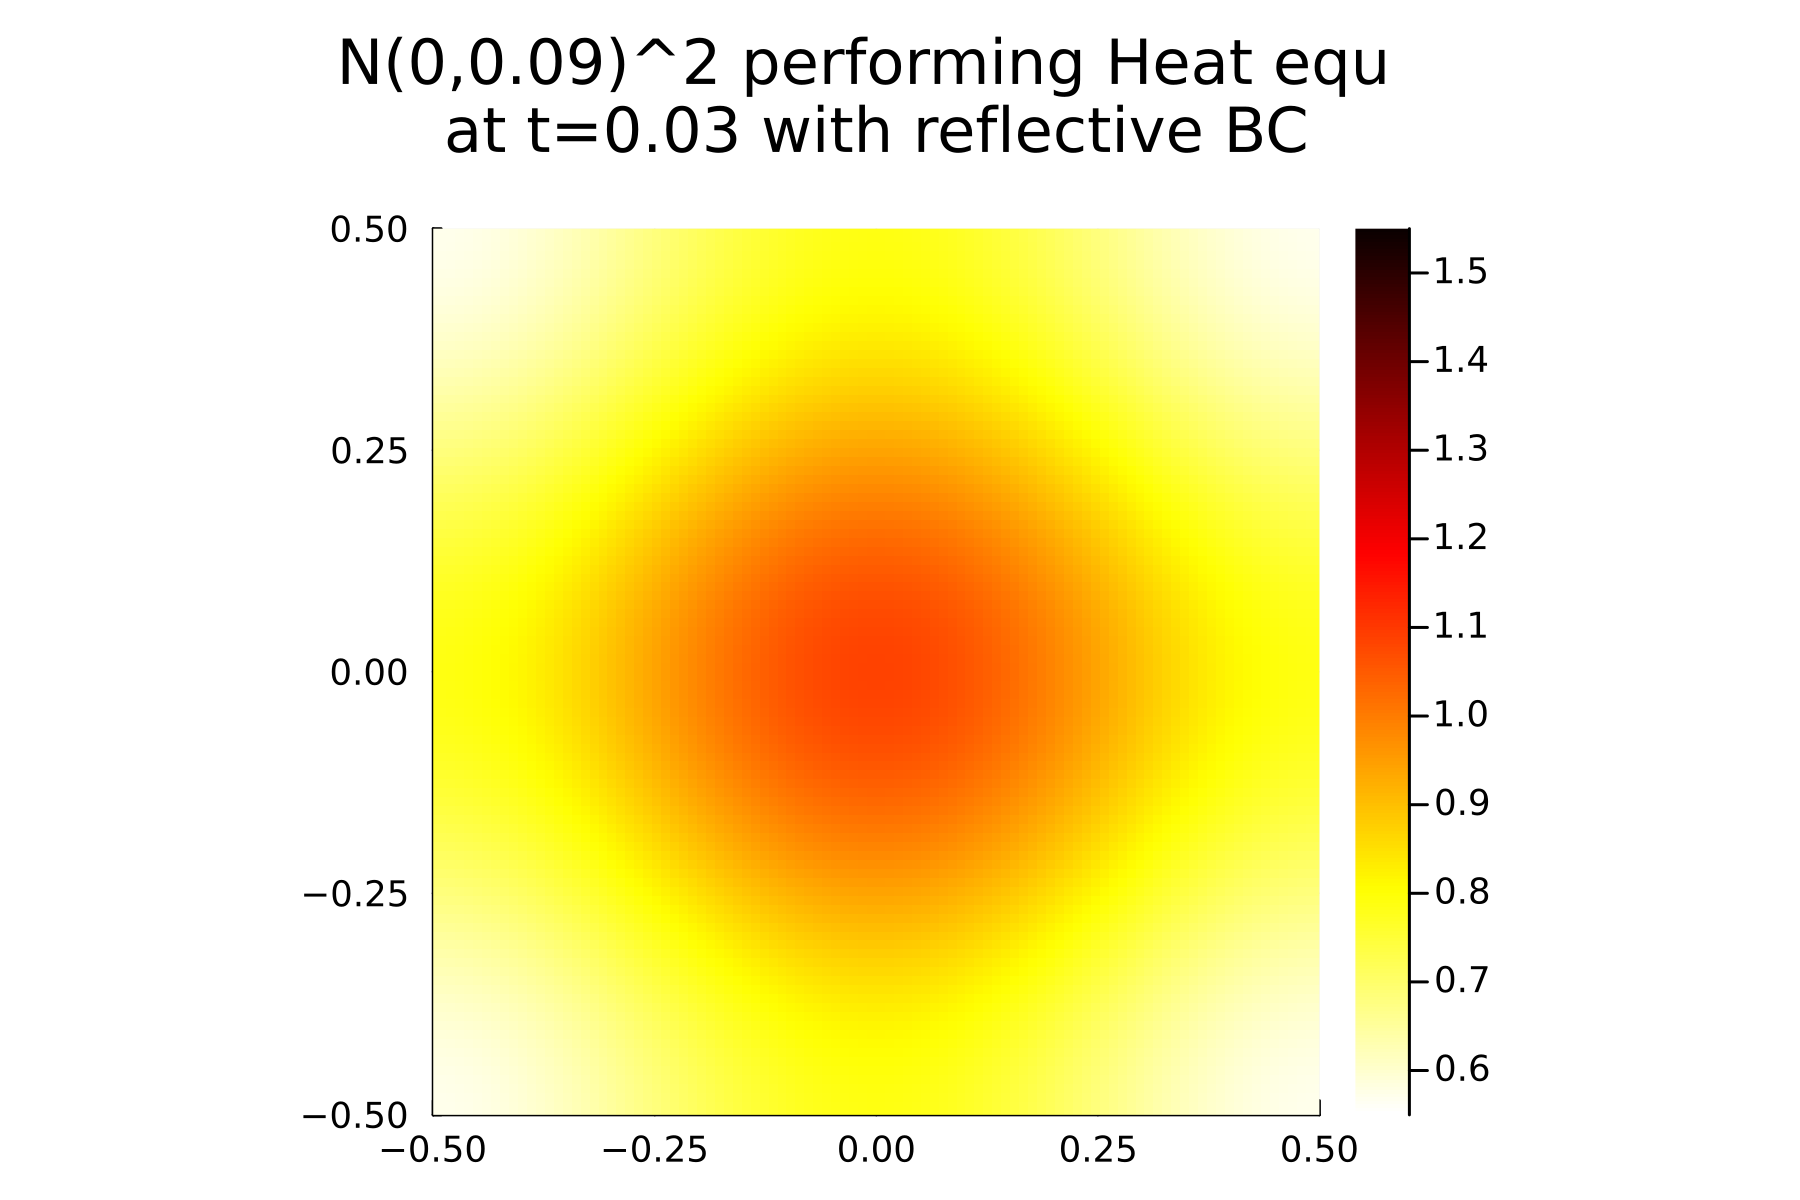
\includegraphics[width=\textwidth]{sanity-check/bruna-scale/heat-dynamic-bruna12-scale-T0-03.png}
% 		\caption{}
% 	\end{subfigure}
% 	\hfill
% 	\begin{subfigure}{0.4\textwidth}
% 		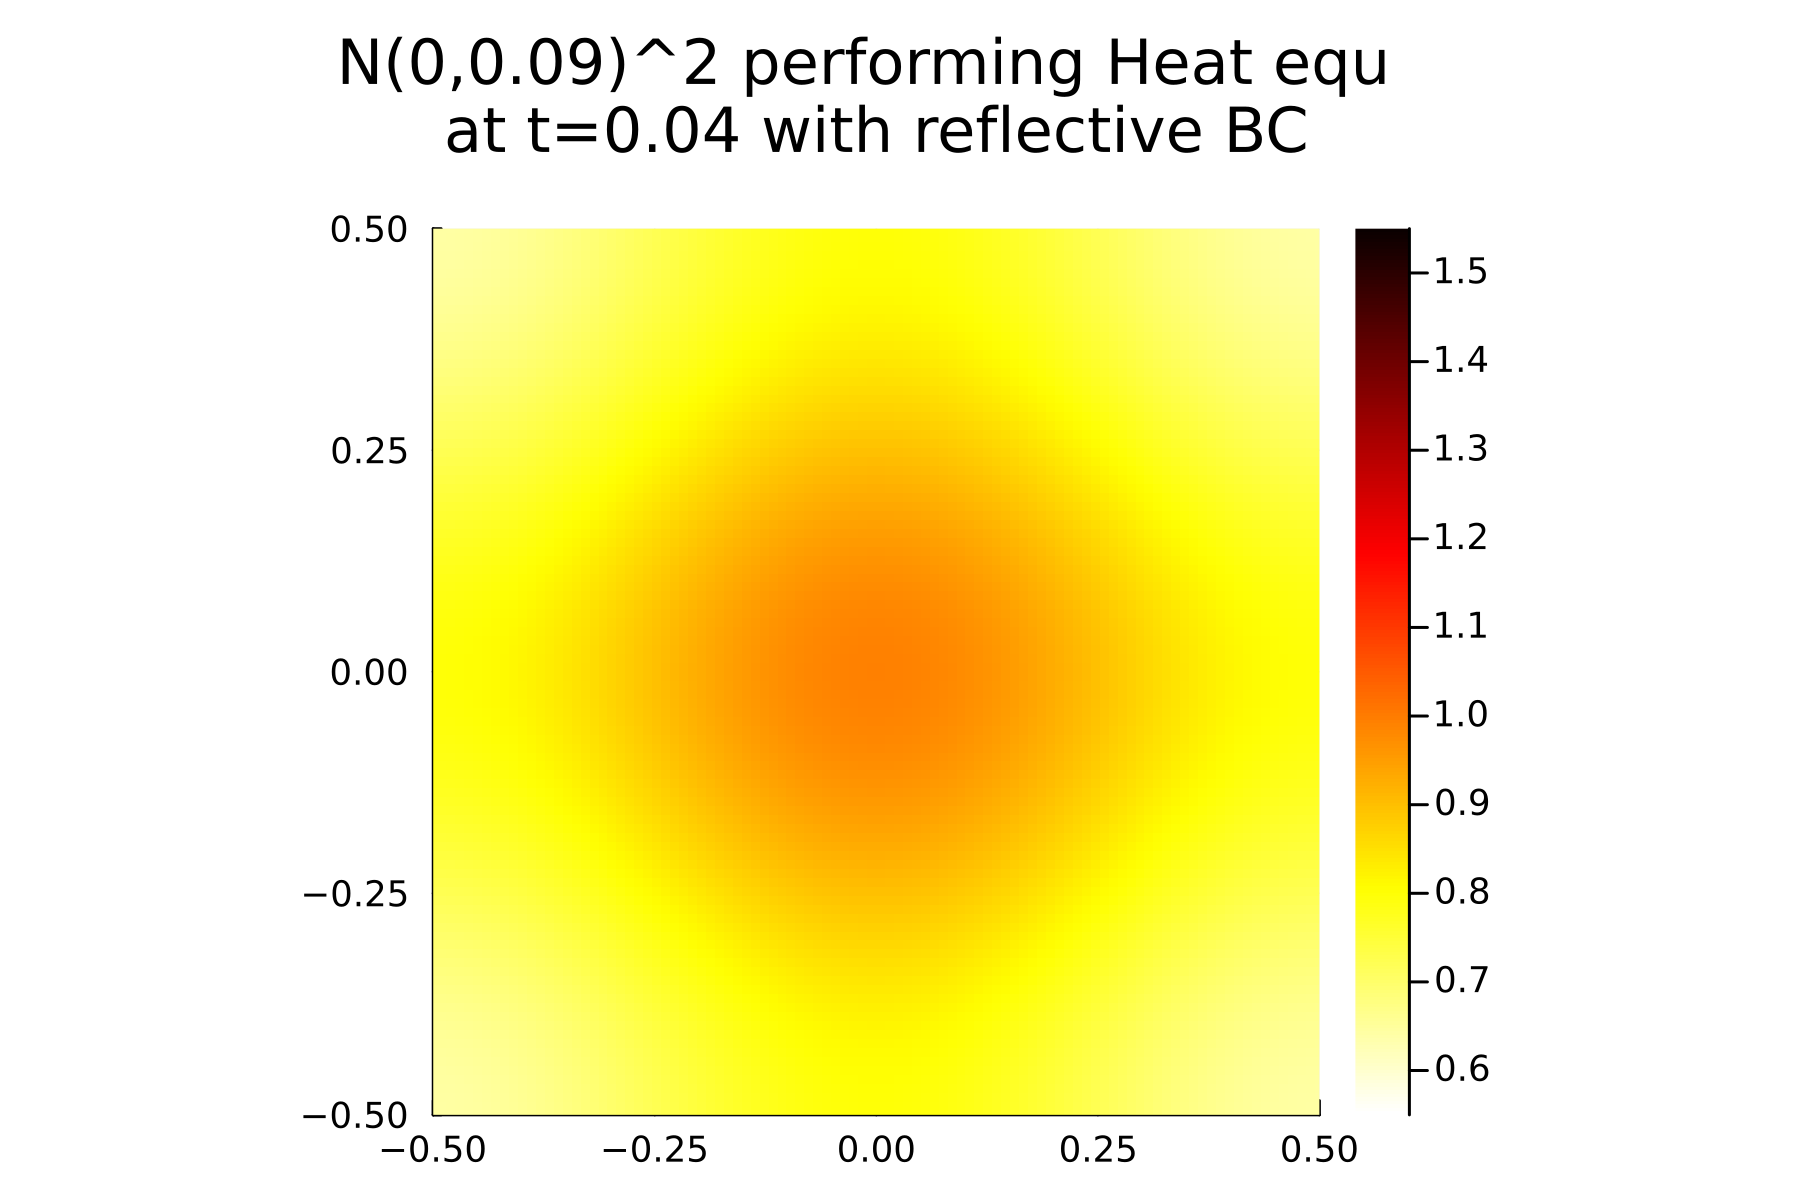
\includegraphics[width=\textwidth]{sanity-check/bruna-scale/heat-dynamic-bruna12-scale-T0-04.png}
% 		\caption{}
% 	\end{subfigure}
%     \begin{subfigure}{0.4\textwidth}
% 		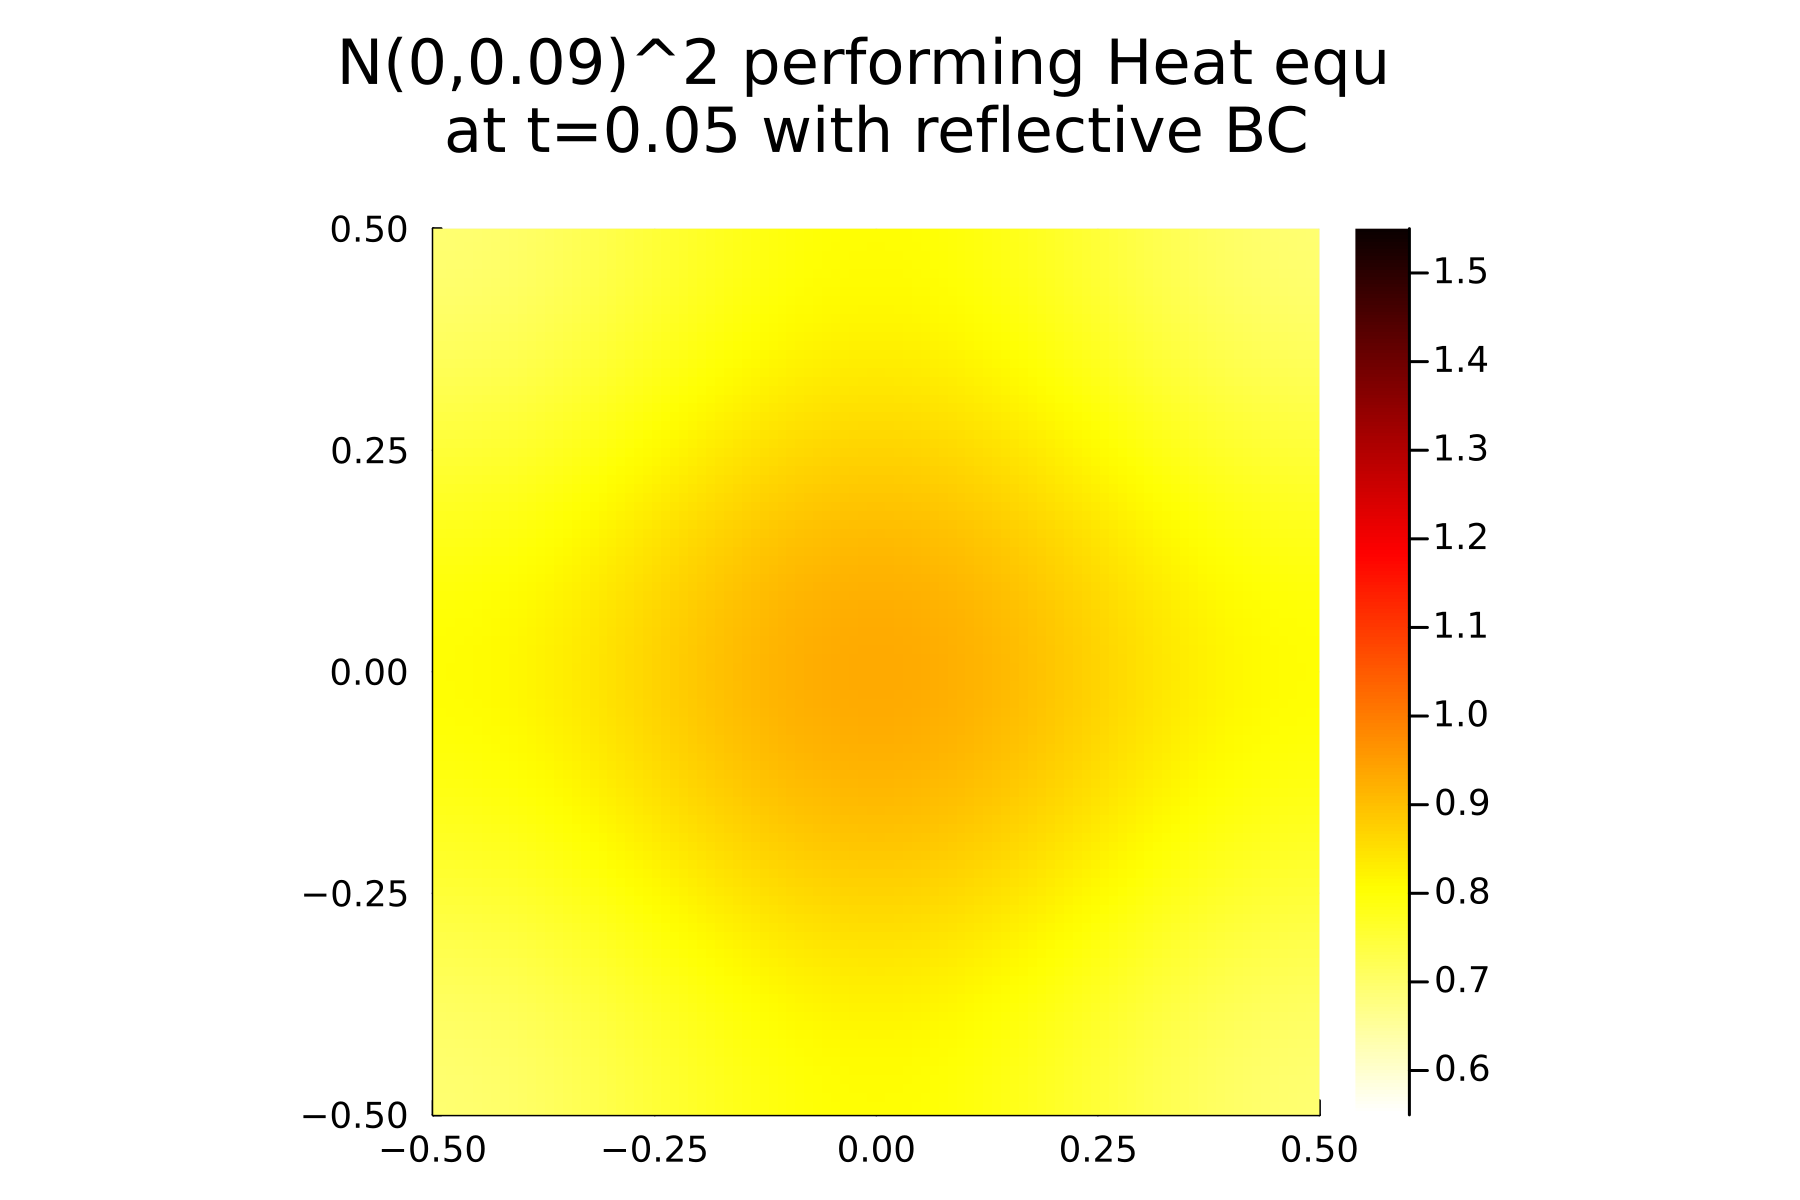
\includegraphics[width=\textwidth]{sanity-check/bruna-scale/heat-dynamic-bruna12-scale-T0-05.png}
% 		\caption{}
% 	\end{subfigure}
% \end{figure}

% \begin{figure}[]
% 	\centering
% 	\begin{subfigure}{0.4\textwidth}
% 		\includegraphics[width=\textwidth]{sanity-check/usual-scale/...}
% 		\caption{}
% 	\end{subfigure}
% 	\hfill
% 	\begin{subfigure}{0.4\textwidth}
% 		\includegraphics[width=\textwidth]{sanity-check/usual-scale/...}
% 		\caption{}
% 	\end{subfigure}
%     \begin{subfigure}{0.4\textwidth}
% 		\includegraphics[width=\textwidth]{sanity-check/usual-scale/...}
% 		\caption{}
% 	\end{subfigure}
% 	\hfill
% 	\begin{subfigure}{0.4\textwidth}
% 		\includegraphics[width=\textwidth]{sanity-check/usual-scale/...}
% 		\caption{}
% 	\end{subfigure}
% \end{figure}




